\section{Moto armonico semplice}
%---------------------------------------------------------------------------
Il moto armonico semplice è un tipo di moto, periodico, che avviene in una
regione confinata dello spazio.\\
Prendiamo il caso in cui un punto materiale che oscilla tra una posizione minima
ed una massima, nel caso più generale possibile possiamo scrivere la sua
legge oraria utilizzando una funzione armonica.

\begin{equation}
    \boxed{x_{(t)} = A\sin\sx \omega t +\phi\dx}
\label{eq:MA}
\end{equation}
\\
Dove $A$ è l'ampiezza di oscillazione, il punto si muove tra $ x = -A$ ed
$x = A$.\\
$\omega$ è la pulsazione, $\omega = 2\pi\nu$ dove $\nu$ è la frequenza ed
indica in numero di oscillazioni effettuate in un secondo.\\
$\phi$ è lo sfasamento iniziale, è collegato alla posizione iniziale tramite:
$ x_0 \coloneqq x_{(0)} = A\sin\phi$\\
Una volta nota la legge oraria è immediato calcolare velocità ed accelerazione,
dato che basta derivare rispetto al tempo.\\
Introduciamo ora una notazione molto utilizzata in fisica ovvero, l'utilizzo
di un punto posto sopra il simbolo di una grandezza per indicarne la
derivata totale rispetto al tempo.

\begin{equation}
    v_{(t)} = \dot x_{(t)} = A\omega\cos\sx\omega t +\phi\dx
\label{eq:MA_velocity}
\end{equation}
\begin{equation}
    a_{(t)} = \dot v_{(t)} = \ddot x_{(t)} = -A\omega^2\sin\sx\omega t +\phi\dx
\label{eq:MA_acceleration}
\end{equation}
\\
Possiamo notare che esiste una relazione tra accelerazione e posizione.

\subsection{Equazione differenziale dell'oscillatore armonico}

Come si può notare chiaramente, l'accelerazione è direttamente proporzionale
alla posizione.

\begin{equation}
    \ddot x = -\omega^2x\seg \boxed{\ddot x_{(t)} + \omega^2x_{(t)} = 0}
\label{eq:DE_armosc}
\end{equation}
\\
La (\ref{eq:DE_armosc}) è un'equazione differenziale al secondo ordine,
a coefficienti costanti, omogenea. Che unita alle due condizioni iniziali:\\
$x_{(0)} = A\sin\phi$ ed $\dot x_{(0)} = A\omega\cos\phi $ ha come soluzione
la (\ref{eq:MA}).\\
Ora che sappiamo che $a_{(x)} = -\omega^2x$ possiamo utilizzare la formula
(\ref{eq:v(x)_gen}) per ottenere $v_{(x)}$.

\begin{equation}
    \boxed{v^2_{(x)} = v_0^2 - \omega^2\sx x^2 - x_0^2\dx}
\label{eq:v(x)_MA}
\end{equation}

\begin{figure}[htbp]
    \begin{center}
        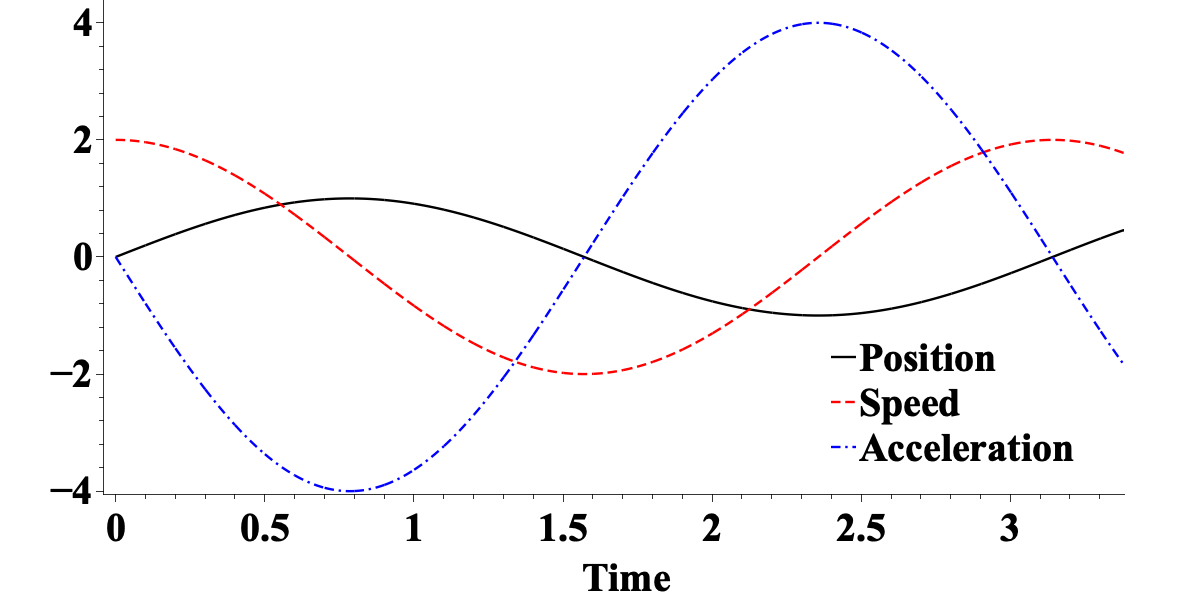
\includegraphics[width=13cm]{images/MA.png} 
        \caption{Un esempio del grafico di accelerazione (blu), velocità
        (rosso) e posizione (nero), nel moto armonico semplice.
        }
    \end{center}
\label{fig:MA}
\end{figure}